% major update 8/4/11
% typo fixes 12/5/11
% --------------------------------------------------------------------------
%\documentclass[onecolumn,11pt]{ieeetran}
\documentclass[]{siamltex}
\usepackage{graphics,amssymb,amsmath,amsfonts,epsfig} % stfloats,
%\usepackage{algorithm}
%\usepackage{algorithmic}
\usepackage{hyperref}
\usepackage{verbatim}
%\usepackage[named]{algo}

% Example definitions
% -------------------
\def\x{{\mathbf x}}
\def\L{{\cal L}}
\def\half{\frac{1}{2}}
\def\alphamax{\alpha_{\mbox{\tiny max}}}
\def\alphamin{\alpha_{\mbox{\tiny min}}}


% more useful abbreviations
% -------------------------
\newcommand{\R}{\mathbb{R}}
\newcommand{\C}{\mathbb{C}}
\newcommand{\btheta}{\mbox{\boldmath $\theta$}}
\newcommand{\bgamma}{\mbox{\boldmath $\gamma$}}
\newcommand{\bbeta}{\mbox{\boldmath  $\beta$}}
\newcommand{\balpha}{\mbox{\boldmath $\alpha$}}
\newcommand{\bDelta}{\mbox{\boldmath $\Delta$}}
\newcommand{\bdelta}{\mbox{\boldmath $\delta$}}
\newcommand{\bPsi}{\mbox{\boldmath   $\Psi$}}
\newcommand{\bphi}{\mbox{\boldmath   $\phi$}}
\newcommand{\bpi}{\mbox{\boldmath    $\pi$}}
\newcommand{\btau}{\mbox{\boldmath   $\tau$}}
\newcommand{\blambda}{\mbox{\boldmath $\lambda$}}
\newcommand{\bTheta}{\mbox{\boldmath $\Theta$}}
\newcommand{\bone}{\mbox{\boldmath   $1$}}
\newcommand{\Loewner}[0]{\preceq}
\newcommand{\Hessmat}{{\cal H}}
\newcommand{\Bmat}{{\bf B}}
\newcommand{\Amat}{{\bf A}}
\newcommand{\bx}{{\bf x}}
\newcommand{\gradv}{{\bf g}}
\newcommand{\cG}{{\cal G}}
\newcommand{\cS}{{\cal S}}
\newcommand{\cT}{{\cal T}}
\newcommand{\trace}{\mbox{\rm trace}}
\newcommand{\tv}{\tilde{v}}
\newcommand{\gammaC}{\gamma_C}

\def\noprint#1{}
\def\swcomment#1{{\em [SW: #1]}}
\def\dmcomment#1{{\em [DM: #1]}}
\def\swresolved#1{}
\def\dmresolved#1{}
\def\sparsa{SpaRSA\ }
\def\bi{\begin{itemize}}
\def\ei{\end{itemize}}
\def\beq{\begin{equation}}
\def\eeq{\end{equation}}
\def\eqnok#1{(\ref{#1})}

% theorem environments
% \newtheorem{theorem}{Theorem}
% \newtheorem{lemma}[theorem]{Lemma}
% \newtheorem{corollary}[theorem]{Corollary}

% baselinestretch definition is important!!
% \renewcommand{\baselinestretch}{1.565}

% \ninept

% Title.
% ------
\title{Discussion 9, \hspace{1.2cm} November 27}

\begin{document}
%\ninept
%
\maketitle

\begin{enumerate}
\item (10 points, 5 points each sub-part.) The continuous-time signal $$x_c(t) = \sin(21 \pi t ) + \cos (35 \pi t)$$ is sampled with a sampling period $T$ to obtain the discrete-time signal $$x[n] = \sin\left(\frac{\pi n}{15}\right) + \cos\left(\frac{\pi n}{9}\right)\;.$$ 
% OSB 2nd edition 4.4

\vspace{5mm} 
	\begin{enumerate}
	\item Determine a choice for $T$ consistent with this information. 
	
	Hint: Write an equation that relates $x[n]$ with $x_c(t)$ through the sampling period $T$.
	
	\vspace{2cm}
	\item Is your choice for $T$ in Part (a) unique? If so, explain why. If not, specify another choice of $T$ consistent with the information given.
	
	Hints:
		\begin{enumerate}
			\item We notice that $x_c(t)$ is periodic. What is the definition of periodicity for continuous time signals? If there exists some positive value, $T_P$, s.t. for all $t$, $x_c(t)=\ldots$
			\item What is the period of $x_c(t)$?
			\item What effect did we notice with the wagon wheel demonstration in class? How does that relate to the period? It may help to draw a simple sine and simulate sampling on it.
		\end{enumerate}
	\end{enumerate}


\newpage
\item (20 points total, see point values below.) The given sequence $x_1[n]$ is periodic with period $N=4$. We would like to convolve it with the $h[n]$ given. 
\vspace{4mm}

\[x_1[n] = \begin{cases} 3,\quad  n \text{ mod }4 = 0\\ 1,\quad  n \text{ mod }4 = 1 \text{ or } 3\\0,\quad  n\text{ mod }4 = 2 \end{cases}\qquad \qquad h[n] = \{\underline{1},-1\} \]

	\begin{enumerate} 
	\item (5 points) What is the result of the length-$N=4$ periodic convolution between these two sequences?
	
	Hint: Write the mathematical of periodic convolution. What does the tilde indicate?
	
	\vspace{3in}
	\item (5 points) Now consider $x_2[n]$, which is zero for all indices not shown. What is the result of the length-$N=4$ circular convolution of $x_2[n]$ and $h[n]$?
	\[ x_2[n] = \{\underline{3},1,0,1 \} \]
	
	Hint: Write the mathematical definition of circular convolution. How does it differ from the definition of periodic convolution in part (a)? Over what values of $n$ is this defined? 
	
	
	\newpage
	\item (10 points) Now consider that we would like to implement the following LTI system, where $H(\omega)$ is the DTFT of $h[n]$ given above.
	
	$$x_2[n]  \rightarrow \fbox{$H(\omega)$} \rightarrow y_2[n]\;.$$
	
	Instead we need to implement it on a computer, so we'll use the DFT as follows. 
	
	$$h[n] \rightarrow \fbox{? \#1} \rightarrow g[n] \rightarrow \fbox{M-point DFT} \rightarrow G[k] $$		
	$$x_2[n] \rightarrow \fbox{? \#2} \rightarrow w[n] \rightarrow \fbox{M-point DFT}  \rightarrow \fbox{$G[k]$}\rightarrow  \fbox{M-point IDFT}  \rightarrow y_2[n]\;.$$
	
		\begin{enumerate} 
		\item What is the minimum value $M$ can be to guarantee we get the linear convolution?
		
		Hint: what is the length of linear convolution?
		\vspace{.5in}
		
		\item Describe what we must do to $x_2[n]$ and/or $h[n]$ (i.e. what should we do at the "?" boxes) to guarantee that $$y_2[n] = x_2[n]*h[n],$$ 
		
		i.e. the output is the linear convolution of $x_2[n]$ and  $h[n]$.
		
		Hint: We are not asking about alternate ways to compute $y_2[n]$- just what needs to go in ?\#1 and ?\#2. Think about part(i).
		
		\vspace{1in} 
		
		
		\item Suppose we took $M=8$. In this case, describe how $G[k]$ relates to $H[k]$, the $N=4$-point DFT of $h[n]$. (You do not have to solve for $H[k]$ and $G[k]$ explicitly, just describe how they relate.)
		
		Hints: 
			\begin{enumerate}
			\item Write down how $H[k]$ and $G[k]$ mathematically relate to $H(e^{j\omega})$. 
			\item Knowing one of the two DFTs can tell you the other, but not vice versa. Why?
			\end{enumerate}
		\end{enumerate}
	\end{enumerate}



\newpage
\item (15 points total, see point values below) Consider the systems shown below. Suppose that $H_1(\omega)$ is fixed and known. 
% OSB 2nd edition 4.29, GATech PS 7 solutions

$$x_1[n] \rightarrow \fbox{$\downarrow 2$} \rightarrow v[n]  \rightarrow \fbox{$H_1(\omega)$}  \rightarrow q[n]\rightarrow \fbox{$\uparrow 2$} \rightarrow y_1[n]\;,$$


\begin{eqnarray*} x_2[n] \rightarrow \fbox{?} \rightarrow \oplus & \rightarrow \fbox{$H_2(\omega)$} \rightarrow y_2[n]  \\
\uparrow & \\
x_2[n] & .
\end{eqnarray*} 

\vspace{3mm} Remember that \fbox{$\uparrow M$} means we insert $M-1$ zeros between samples and \fbox{$\downarrow M$} means we take every $M^{th}$ sample.

\vspace{3mm} 
	\begin{enumerate}
	\item (5 points) What is $V(\omega)$ in terms of $X_1(\omega)$? What is $Q(\omega)$ in terms of $X_1(\omega)$ and $H_1(\omega)$?
	
	Hint: What is $Q(\omega)$ in terms of $V(\omega)$ and $H_1(\omega)$?
	
	\vspace{2cm} \item (10 points) Find $H_2(\omega)$, the frequency response of an LTI system and the operation that belongs in the "?" box, such that $y_1[n] = y_2[n]$ when $x_1[n] = x_2[n]$ (in other words, the outputs are the same when the inputs are the same).
	
	Hints: \begin{enumerate}
			\item Start by writing out $Y_1(\omega)$ in terms of $Q(\omega)$ and then in terms of $X_1(\omega)$ and $H_1(\omega)$.
			\item For the "?" box, use an idea from problem 5.
			\end{enumerate}
	
	\end{enumerate}



\newpage
\item (15 points) For the FFT, we learned how to break a length-8 DFT into two DFTs of length-4. Use the same approach to show how you could break a length-20 DFT into five DFTs of length-4. 

Hint: Start with the definition of the DFT and think about ways to divide the summation into three different interleaved summations.






\newpage

\item (30 points total, plus 5 points extra credit, see point values below.) 
% OSB 4.38 2nd edition, Solution in SP05_PS7_soln of GA Tech
	\begin{enumerate}
	\item (12 points) Consider the following system. $$x_c(t)  \rightarrow \fbox{C/D with period $T$}  \rightarrow x[n] \rightarrow   \fbox{$H(\omega)$} \rightarrow v[n] \rightarrow \fbox{$\downarrow L$} \rightarrow q[n] $$
	
	The filter $H(\omega)$ is defined as $$H(\omega) = \left\{ \begin{matrix} 1, & |\omega| < \pi/L \\ 0 , & \pi/L < |\omega| < \pi\end{matrix} \right. \;.$$
	
	$X_c(\Omega)$ is given in this figure. What do $V(\omega)$ and $Q(\omega)$ look like? Draw them on a plot with clear labels of the axes, the locations where the signal touches the x-axis, and the height of the signal.
	
	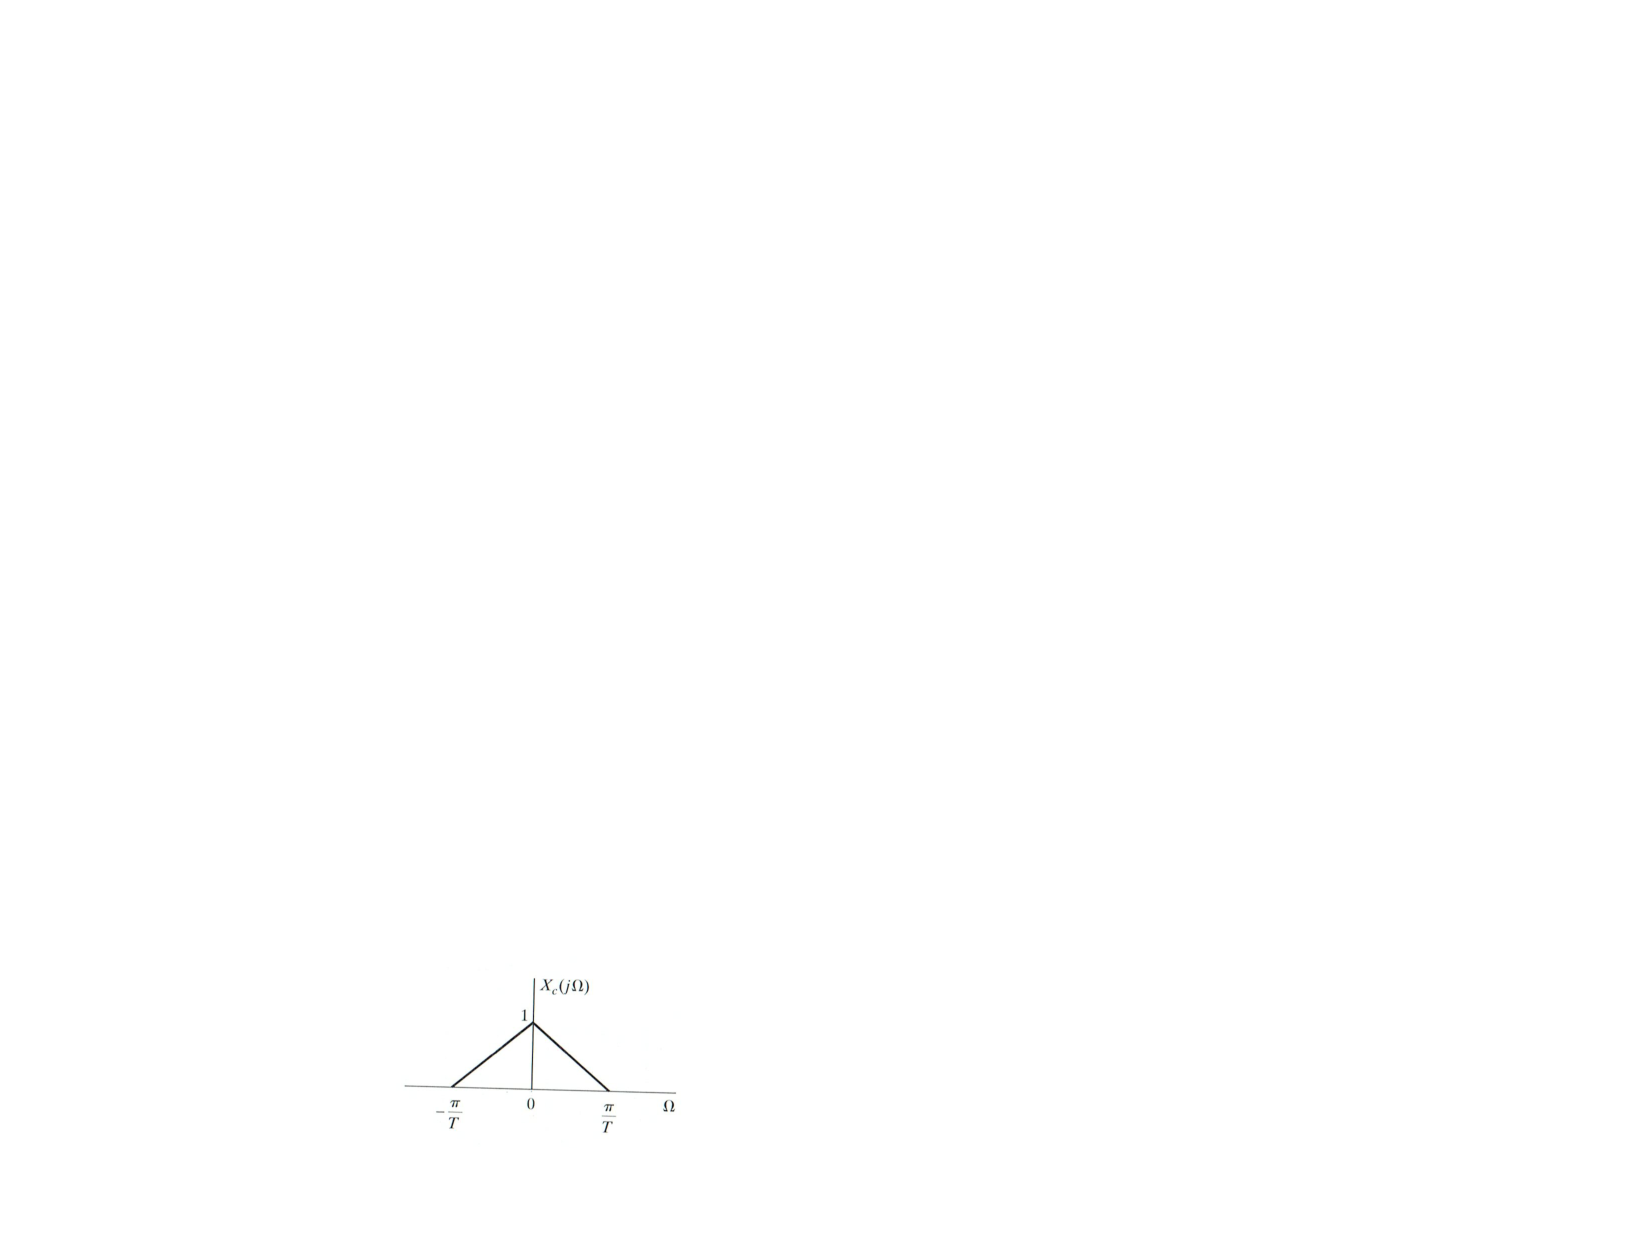
\includegraphics{osb4382}
	
		Hints: 
		\begin{enumerate}
			\item Follow the instructions! Label everything!
			\item Write out the formula that relates $X_c(\Omega)$ to $X(\omega)$ through sampling period $T$. Pay attention to scaling in both the domain and the amplitude.
		\end{enumerate}
	
	\newpage
	\item (18 points) Now continue the system from part (a) as follows, where $q[n]$ is the output of the system in part (a).
	
	$$q[n] \rightarrow \fbox{Modulator} \rightarrow y[n] \rightarrow  \fbox{D/C with period $T' = LT$} \rightarrow y_c(t)$$
	
	
	The box labeled ``Modulator'' takes the input sequence $q[n]$ and multiplies it by $j^n$: $$y[n] = j^n q[n]\;.$$ Draw $Y(\omega)$, the DTFT of $y[n]$, and $Y_c(\Omega)$, the CTFT of $y_c(t)$. Again be sure to clearly label the axes, locations where the signal touches the x-axis, and the height of the signal.
	
	Hints: 
		\begin{enumerate}
			\item $j^n$ can be alternatively expressed as $(?)^n$ (think polar coordinates in the complex plane). What DTFT property is useful here?
			\item Write the formula that relates $Y_c(\Omega)$ to $Y(\omega)$ through the interpolation period $T'$. (You've already had to use it in this problem.)
		\end{enumerate}
	
	\vspace{4in}
	\item (5 points, extra credit) Can we swap the modulator with our LTI filter $H(\omega)$ and still get the same overall system? Why or why not?
	
	Hint: You won't be able to get any extra credits points back but draw some pictures and test it out for yourself. :)
	\end{enumerate}








\end{enumerate}


\end{document}
